\documentclass[../../main.tex]{subfiles}

\graphicspath{{\subfix{../../immagini/}}}

\begin{document}
    Vengono ora presentati i risultati ottenuti inserendo le due categorie di classificatore all'interno dei filtri appresi. Come brevemente spiegato nel paragrafo \ref{sec:Esperimenti}, i risultati del precedente paragrafo posso essere utilizzati solamente per fornire un'idea dell'efficacia dei classificatori nel problema di riconoscimento degli URL; in questo secondo blocco di esperimenti, infatti, l'obiettivo è trovare il classificatore che porti alla maggiore diminuzione in termini di spazio dei filtri. Di fatto vogliamo quindi cercare un tradeoff tra prestazioni e spazio occupato.

    Il classificatore migliore in questo caso non può essere trovato tramite una classica model selection: nessuna metrica, infatti, risulta adatta a quantificare la bontà di un modello in termini di spazio occupato. Una model selection risulterebbe di conseguenza inadatta perché non avremmo nessuna metrica da massimizzare.

    Il numero di neuroni del percettrone viene quindi scelto in modo da ottenere un modello con una taglia molto vicina a quella della GRU a 16 dimensioni. Inoltre, dai risultati dello scorso paragrafo è possibile notare come, aumentando di molto il numero di neuroni, l'aumento delle prestazioni non sia altrettanto significativo. Per questo motivo viene testato un ulteriore modello con un numero inferiore di neuroni, scelto arbitrariamente, al fine di evidenziare eventuali miglioramenti nella dei taglia filtri appresi dovuti ad una dimensione minore del modello.

    Secondo questo ragionamento, viene testata una configurazione con 30 neuroni, che ha una grandezza molto simile alla GRU 16, e una configurazione con 20 neuroni. In entrambi casi il learning rate viene fissato a 0.001, dai risultati del precedente paragrafo sembra infatti la scelta migliore.
    
    \subsubsection{Scelta della soglia $\tau$}
    Una volta scelti a priori il tasso di falsi positivi desiderato $f$ e il tasso di falsi positivi del classificatore, in questo paragrafo chiamato $f_{\tau}$, la soglia $\tau$ ha un valore pari al quantile $100 \cdot (1 - f_{\tau})$ della distribuzione di probabilità, ritornata dal classificatore, delle non-chiavi presenti nell'insieme d'addestramento.

    Coerentemente con quanto detto nel paragrafo \ref{sec:falseProbLBF}, vengono testati diversi valori di $\tau$ variando il valore del rapporto $r_{\tau} = f_{\tau}/f$. Importante notare che, a seconda  del filtro considerato, dovranno valere le condizioni su $f_{\tau}$ descritte nel capitolo \ref{chap:filtriAppresi}.

    \subsubsection{Risultati filtro di Bloom}

    Vengono riportate in tabella \ref{tab:taglieFiltro} le taglie dei filtri di Bloom inizializzati sull'insieme delle chiavi $\mathcal{K}$, queste verranno utilizzate come base per confrontare le performance dei filtri appresi riportate successivamente.

    Una volta fissato $f$, le taglie sono state calcolate secondo l'equazione \ref{eqn:nlowerbound}.
    
    \begin{table}
        \centering
        \begin{tabular}{lcccc}
            \toprule
            {} & \multicolumn{4}{c}{\textbf{FPR $f$}}\\
            {} & 0.001 & 0.005 & 0.01 & 0.02\\
            \midrule
            \textbf{Dimensione (KByte)} & 76.774 & 58.887 & 51.212 & 43.479\\
            \bottomrule
        \end{tabular}
        \caption{Taglie dei filtri di Bloom.}
        \label{tab:taglieFiltro}
    \end{table}

    \subsubsection{Risultati LBF}
    Le figure \ref{fig:percettroneEmpiricoLBF} e \ref{fig:GRUEmpiricoLBF} mostrano graficamente i risultati delle analisi empiriche, al variare del rapporto $r_{\tau}$, delle due tipologie di classificatore; la figure \ref{fig:tagliePercettroniLBF} e \ref{fig:taglieGRULBF}, invece, mostrano le taglie dell'intero LBF. In questo caso deve valere $0 < r_{\tau} < 1$, il rapporto viene quindi fatto variare tra questi due valori.

    Nello specifico, le figure \ref{fig:LBFFNRPercettrone20} e \ref{fig:LBFFNRPercettrone30} per il percettrone, e \ref{fig:LBFFNR_GRU16}, \ref{fig:LBFFNR_GRU8} e \ref{fig:LBFFNR_GRU4} per la GRU, mostrano il tasso di falsi negativi prodotti dal classificatore al variare del rapporto $r_{\tau}$. Si nota in tutte le figure una diminuzione del rapporto di falsi negativi all'aumentare di $r_{\tau}$, ciò è sensato: all'aumentare di $r_{\tau}$ il valore della soglia $\tau$ diminuisce, di conseguenza è più probabile che una chiave venga classificata come tale, generando un numero di falsi negativi via via minore.

    \begin{figure}[H]
        \centering
        \begin{subfigure}[b]{0.49\textwidth}
            \centering
            \includegraphics[width = \textwidth]{immagini/7/LBF/Percettrone(20, 0.001)_FNR.png}
            \caption{Rapporto dei falsi negativi prodotti dal percettrone (20, 0.001).}
            \label{fig:LBFFNRPercettrone20}
        \end{subfigure}
        \begin{subfigure}[b]{0.49\textwidth}
            \centering
            \includegraphics[width = \textwidth]{immagini/7/LBF/Percettrone(30, 0.001)_FNR.png}
            \caption{Rapporto dei falsi negativi prodotti dal percettrone (30, 0.001).}
            \label{fig:LBFFNRPercettrone30}
        \end{subfigure}
        \begin{subfigure}[b]{0.49\textwidth}
            \centering
            \includegraphics[width = \textwidth]{immagini/7/LBF/Percettrone(20, 0.001)_FPR.png}
            \caption{Tasso empirico di falsi positivi del percettrone (20, 0.001).}
            \label{fig:LBFFPRPercettrone20}
        \end{subfigure}
        \begin{subfigure}[b]{0.49\textwidth}
            \centering
            \includegraphics[width = \textwidth]{immagini/7/LBF/Percettrone(30, 0.001)_FPR.png}
            \caption{Tasso empirico di falsi positivi del percettrone (30, 0.001).}
            \label{fig:LBFFPRPercettrone30}
        \end{subfigure}
        \caption{Misurazioni empiriche sui percettroni.}
        \label{fig:percettroneEmpiricoLBF}
    \end{figure}

    \begin{figure}[H]
        \centering
        \begin{subfigure}[b]{0.32\textwidth}
            \centering
            \includegraphics[width = \textwidth]{immagini/7/LBF/GRU16_FNR.png}
            \caption{Rapporto dei falsi negativi prodotti dalla GRU 16.}
            \label{fig:LBFFNR_GRU16}
        \end{subfigure}
        \begin{subfigure}[b]{0.32\textwidth}
            \centering
            \includegraphics[width = \textwidth]{immagini/7/LBF/GRU8_FNR.png}
            \caption{Rapporto dei falsi negativi prodotti dalla GRU 8.}
            \label{fig:LBFFNR_GRU8}
        \end{subfigure}
        \begin{subfigure}[b]{0.32\textwidth}
            \centering
            \includegraphics[width = \textwidth]{immagini/7/LBF/GRU4_FNR.png}
            \caption{Rapporto dei falsi negativi prodotti dalla GRU 4.}
            \label{fig:LBFFNR_GRU4}
        \end{subfigure}
        \begin{subfigure}[b]{0.32\textwidth}
            \centering
            \includegraphics[width = \textwidth]{immagini/7/LBF/GRU16_FPR.png}
            \caption{Tasso empirico di falsi positivi della GRU 16.}
            \label{fig:LBFFPR_GRU16}
        \end{subfigure}
        \begin{subfigure}[b]{0.32\textwidth}
            \centering
            \includegraphics[width = \textwidth]{immagini/7/LBF/GRU8_FPR.png}
            \caption{Tasso empirico di falsi positivi della GRU 8.}
            \label{fig:LBFFPR_GRU8}
        \end{subfigure}
        \begin{subfigure}[b]{0.32\textwidth}
            \centering
            \includegraphics[width = \textwidth]{immagini/7/LBF/GRU4_FPR.png}
            \caption{Tasso empirico di falsi positivi della GRU 4.}
            \label{fig:LBFFPR_GRU4}
        \end{subfigure}
        \caption{Misurazioni empiriche sulle GRU.}
        \label{fig:GRUEmpiricoLBF}
    \end{figure}

    Le figure \ref{fig:LBFFPRPercettrone20}, \ref{fig:LBFFPRPercettrone30}, \ref{fig:LBFFPR_GRU16}, \ref{fig:LBFFPR_GRU8} e \ref{fig:LBFFPR_GRU4}, invece, mostrano il tasso di falsi positivi $f$ dell'intero LBF, calcolato sull'insieme di test composto di soli URL legittimi. In questo caso, come previsto, il tasso empirico rimane sempre stabile attorno al tasso atteso.

    Infine, le figure \ref{fig:LBFTagliaPercettrone20}, \ref{fig:LBFTagliaPercettrone30}, \ref{fig:LBFTagliaGRU16}, \ref{fig:LBFTagliaGRU8} e \ref{fig:LBFTagliaGRU4} mostrano le taglie dei rispettivi classificatori al variare di $r_{\tau}$. Confrontando i risultati di percettrone e GRU si nota come, in tutti i casi, le due configurazioni di percettrone occupino uno spazio inferiore rispetto alle GRU. Inoltre, è facile notare che i filtri appresi con GRU non siano quasi mai migliori rispetto ai corrispettivi filtri di Bloom, al contrario, i percettroni sembrano occupare uno spazio minore rispetto ai relativi filtri. 

    Confrontando invece le taglie occupate dalle due configurazioni di percettrone, si nota come il modello a 20 neuroni sembri leggermente migliore rispetto a quello a 30. Questo conferma quanto supposto inizialmente: seppur il modello a 30 neuroni sia migliore, in termini di performance, rispetto a quello a 20, quest'ultimo risulta migliore se inserito all'interno di un filtro appreso. Le performance guadagnate, non sono quindi sufficienti a giustificare l'aumento di spazio del modello.

    \begin{figure}[H]
        \centering
        \begin{subfigure}[b]{0.49\textwidth}
            \centering
            \includegraphics[width = \textwidth]{immagini/7/LBF/Percettrone(20, 0.001)_Taglia.png}
            \caption{Taglia del percettrone (20, 0.001)}
            \label{fig:LBFTagliaPercettrone20}
        \end{subfigure}
        \begin{subfigure}[b]{0.49\textwidth}
            \centering
            \includegraphics[width = \textwidth]{immagini/7/LBF/Percettrone(30, 0.001)_Taglia.png}
            \caption{Taglia del percettrone (30, 0.001)}
            \label{fig:LBFTagliaPercettrone30}
        \end{subfigure}
        \caption{Taglie dei percettroni.}
        \label{fig:tagliePercettroniLBF}
    \end{figure}

    \begin{figure}[H]
        \centering
        \begin{subfigure}[b]{0.32\textwidth}
            \centering
            \includegraphics[width = \textwidth]{immagini/7/LBF/GRU16_Taglia.png}
            \caption{Taglia della GRU 16.}
            \label{fig:LBFTagliaGRU16}
        \end{subfigure}
        \begin{subfigure}[b]{0.32\textwidth}
            \centering
            \includegraphics[width = \textwidth]{immagini/7/LBF/GRU8_Taglia.png}
            \caption{Taglia della GRU 8.}
            \label{fig:LBFTagliaGRU8}
        \end{subfigure}
        \begin{subfigure}[b]{0.32\textwidth}
            \centering
            \includegraphics[width = \textwidth]{immagini/7/LBF/GRU4_Taglia.png}
            \caption{Taglia della GRU 4.}
            \label{fig:LBFTagliaGRU4}
        \end{subfigure}
        \caption{Taglie delle GRU.}
        \label{fig:taglieGRULBF}
    \end{figure}

    \subsubsection{Risultati SLBF}
    Anche in questo caso nelle figure \ref{fig:percettroneEmpiricoSLBF} e \ref{fig:GRUEmpiricoSLBF} vengono presentati i risultati empirici sulle strutture, nelle figure \ref{fig:tagliePercettroniSLBF} e \ref{fig:taglieGRUSLBF}, invece, le rispettive taglie. In questo caso $r_{\tau}$ viene fatto variare nell'intervallo $(1 - m_b/m) \leq r_{\tau} \leq 1/f \cdot \left(1 - m_b/m\right)$.
    \begin{figure}[H]
        \centering
        \begin{subfigure}[b]{0.49\textwidth}
            \centering
            \includegraphics[width = \textwidth]{immagini/7/SLBF/Percettrone(20, 0.001)_FNR.png}
            \caption{Rapporto dei falsi negativi prodotti dal Percettrone (20, 0.001).}
            \label{fig:SLBFFNRPercettrone20}
        \end{subfigure}
        \begin{subfigure}[b]{0.49\textwidth}
            \centering
            \includegraphics[width = \textwidth]{immagini/7/SLBF/Percettrone(30, 0.001)_FNR.png}
            \caption{Rapporto dei falsi negativi prodotti dal Percettrone (30, 0.001).}
            \label{fig:SLBFFNRPercettrone30}
        \end{subfigure}
        \begin{subfigure}[b]{0.49\textwidth}
            \centering
            \includegraphics[width = \textwidth]{immagini/7/SLBF/Percettrone(20, 0.001)_FPR.png}
            \caption{Tasso empirico di falsi positivi del Percettrone (20, 0.001).}
            \label{fig:SLBFFPRPercettrone20}
        \end{subfigure}
        \begin{subfigure}[b]{0.49\textwidth}
            \centering
            \includegraphics[width = \textwidth]{immagini/7/SLBF/Percettrone(30, 0.001)_FPR.png}
            \caption{Tasso empirico di falsi positivi del Percettrone (30, 0.001).}
            \label{fig:SLBFFPRPercettrone30}
        \end{subfigure}
        \caption{Misurazioni empiriche sui percettroni.}
        \label{fig:percettroneEmpiricoSLBF}
    \end{figure}

    \begin{figure}[H]
        \centering
        \begin{subfigure}[b]{0.32\textwidth}
            \centering
            \includegraphics[width = \textwidth]{immagini/7/SLBF/GRU16_FNR.png}
            \caption{Rapporto dei falsi negativi prodotti dalla GRU 16.}
            \label{fig:SLBFFNR_GRU16}
        \end{subfigure}
        \begin{subfigure}[b]{0.32\textwidth}
            \centering
            \includegraphics[width = \textwidth]{immagini/7/SLBF/GRU8_FNR.png}
            \caption{Rapporto dei falsi negativi prodotti dalla GRU 8.}
            \label{fig:SLBFFNR_GRU8}
        \end{subfigure}
        \begin{subfigure}[b]{0.32\textwidth}
            \centering
            \includegraphics[width = \textwidth]{immagini/7/SLBF/GRU4_FNR.png}
            \caption{Rapporto dei falsi negativi prodotti dalla GRU 4.}
            \label{fig:SLBFFNR_GRU4}
        \end{subfigure}
        \begin{subfigure}[b]{0.32\textwidth}
            \centering
            \includegraphics[width = \textwidth]{immagini/7/SLBF/GRU16_FPR.png}
            \caption{Tasso empirico di falsi positivi della GRU 16.}
            \label{fig:SLBFFPR_GRU16}
        \end{subfigure}
        \begin{subfigure}[b]{0.32\textwidth}
            \centering
            \includegraphics[width = \textwidth]{immagini/7/SLBF/GRU8_FPR.png}
            \caption{Tasso empirico di falsi positivi della GRU 8.}
            \label{fig:SLBFFPR_GRU8}
        \end{subfigure}
        \begin{subfigure}[b]{0.32\textwidth}
            \centering
            \includegraphics[width = \textwidth]{immagini/7/SLBF/GRU4_FPR.png}
            \caption{Tasso empirico di falsi positivi della GRU 4.}
            \label{fig:SLBFFPR_GRU4}
        \end{subfigure}
        \caption{Misurazioni empiriche sulle GRU.}
        \label{fig:GRUEmpiricoSLBF}
    \end{figure}

    Il ragionamento già fatto per gli LBF può essere ripetuto anche in questo caso: il tasso di falsi positivi del classificatore diminuisce all'aumentare di $r_{\tau}$.

    \begin{figure}[H]
        \centering
        \begin{subfigure}[b]{0.49\textwidth}
            \centering
            \includegraphics[width = \textwidth]{immagini/7/SLBF/Percettrone(20, 0.001)_Taglia.png}
            \caption{Taglia del percettrone (20, 0.001)}
            \label{fig:SLBFTagliaPercettrone20}
        \end{subfigure}
        \begin{subfigure}[b]{0.49\textwidth}
            \centering
            \includegraphics[width = \textwidth]{immagini/7/SLBF/Percettrone(30, 0.001)_Taglia.png}
            \caption{Taglia del percettrone (30, 0.001)}
            \label{fig:SLBFTagliaPercettrone30}
        \end{subfigure}
        \caption{Taglie dei percettroni.}
        \label{fig:tagliePercettroniSLBF}
    \end{figure}

    \begin{figure}[H]
        \centering
        \begin{subfigure}[b]{0.32\textwidth}
            \centering
            \includegraphics[width = \textwidth]{immagini/7/SLBF/GRU16_Taglia.png}
            \caption{Taglia della GRU 16.}
            \label{fig:SLBFTagliaGRU16}
        \end{subfigure}
        \begin{subfigure}[b]{0.32\textwidth}
            \centering
            \includegraphics[width = \textwidth]{immagini/7/SLBF/GRU8_Taglia.png}
            \caption{Taglia della GRU 8.}
            \label{fig:SLBFTagliaGRU8}
        \end{subfigure}
        \begin{subfigure}[b]{0.32\textwidth}
            \centering
            \includegraphics[width = \textwidth]{immagini/7/SLBF/GRU4_Taglia.png}
            \caption{Taglia della GRU 4.}
            \label{fig:SLBFTagliaGRU4}
        \end{subfigure}
        \caption{Taglie delle GRU.}
        \label{fig:taglieGRUSLBF}
    \end{figure}
    \subsubsection{Tempi}

\end{document}